\documentclass[english]{report}


\setlength {\marginparwidth }{2cm} 
\usepackage{todonotes}

\usepackage[perpage,para,symbol]{footmisc}

\hyphenpenalty=15000 
\tolerance=1000

\usepackage{tikz}
\usetikzlibrary{arrows,decorations.pathmorphing,backgrounds,fit,positioning,calc,shapes}
\usepackage{pgfmath}
\usepackage{rotating}
\usepackage{array}	
\usepackage{graphicx}
\usepackage{float}	
\usepackage{mdwlist}
\usepackage{setspace}
\usepackage{listings}
\usepackage{bytefield}
\usepackage{tabularx}
\usepackage{multirow}	       
\usepackage{caption} 
\captionsetup[table]{skip=10pt}

\usepackage{url}               
\usepackage{hyperref}
\usepackage[all]{hypcap}	
\usepackage{titlesec}
\setcounter{secnumdepth}{4}
\titleformat{\paragraph}
{\normalfont\normalsize\bfseries}{\theparagraph}{1em}{}
\titlespacing*{\paragraph}
{0pt}{3.25ex plus 1ex minus .2ex}{1.5ex plus .2ex}
\hypersetup{colorlinks,breaklinks,
            linkcolor=darkblue,urlcolor=darkblue,
            anchorcolor=darkblue,citecolor=darkblue}


\definecolor{darkblue}{rgb}{0.0,0.0,0.3} 
\definecolor{darkred}{rgb}{0.4,0.0,0.0}
\definecolor{red}{rgb}{0.7,0.0,0.0}
\definecolor{lightgrey}{rgb}{0.8,0.8,0.8} 
\definecolor{grey}{rgb}{0.6,0.6,0.6}
\definecolor{darkgrey}{rgb}{0.4,0.4,0.4}
\definecolor{aqua}{rgb}{0.0, 1.0, 1.0}
\definecolor{dkgreen}{rgb}{0,0.6,0}
\definecolor{gray}{rgb}{0.5,0.5,0.5}
\definecolor{mauve}{rgb}{0.58,0,0.82}

\lstset{
  language=C,
  showstringspaces=false,
  columns=flexible,
  basicstyle={\small\ttfamily},
  numbers=none,
  numberstyle=\tiny\color{gray},
  keywordstyle=\color{blue},
  commentstyle=\color{dkgreen},
  stringstyle=\color{mauve},
  breaklines=true,
  breakatwhitespace=true,
  tabsize=3
}
\usepackage{listings}
\PassOptionsToPackage{USenglish,english}{babel} 
\usepackage{csquotes}
\usepackage[USenglish,english]{babel}
\usepackage[acronym, section=section, nonumberlist, nomain, nopostdot]{glossaries}
\makeglossaries
 
\makeglossaries
\newcommand{\colorbitbox}[3]{%
	\rlap{\bitbox{#2}{\color{#1}\rule{\width}{\height}}}%
	\bitbox{#2}{#3}}

\begin{document}

\title{Ethics}

\maketitle

\chapter*{Ethical aspects of autonomous vehicles}
\section*{a. Moral Machine Experiment}

\begin{center}
  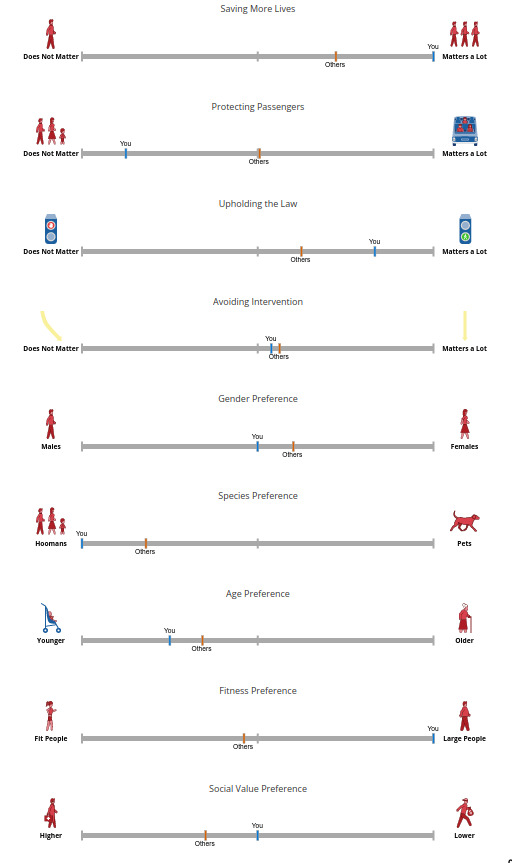
\includegraphics[scale=0.4]{results.jpeg}
\end{center}

\noindent
The online test is a pretty classical test of ethics when it comes to autonomous decision making and implications on life. I think that we are not ready for this step in the sense of ethics, however, a human being would judge this in real life if it happens, thus one should impose a decision making system for computers as well. My decisions were barely based on the metrics they presented, but instead on the law respecting people and almost always on having people in the car considered as ``culprits''.

\section*{c. Reflections on the answers}

I think that mostly, my results might be in the cluster ``Western'', however regarding the lawfullness of the people, my results are more ``Eastern''. I think that even if my results would be classified in any cultural background, for example religion, the best classification is ``Protestant'', however I don't think my results together with the cultural bias it is categorized in do reflect something important to me personally, since I don't find them related in my personality.

\section*{d. Ethics of Autonomous Vehicles}

The situations presented in the experiment are really relevant to everyday life, since they are plausible problems and situations in which an autonomous system might find itself in. However, one thing that should be mentioned is the fact that the technology is not sufficiently advanced in order to take all of the problems of the situation into consideration: it can not know the age of each person, the background and so on, thus these can not be taken into accound in a decision making system. The most one could do is to calculate the number of victims and try to minimize it.\\\\

\noindent
Autonomous vehicles, however, are closer to reality than we think they are. In this sense, a good basis for laws and ethical decisions should be established. For example, a situation when a car does not recognize a red light and runs through it while killing 2 pedestrians because of that is a situation where law should be enforced, but on who? Who is ethically responsible for this?

\section*{e. Essential Design Principles}

First of all, I personally think that problems such as the one exemplified in the test before should be mostly put on the persons in the car. That is, a car owner should be liable to regularly check on his car and the proper functionality of it, regarding consumables and the quality of these over time, such as breaks and how well they are functioning. \\\\

\noindent
I think that in most of the situations, whenever a car is put in front of a case where it could run over pedestrians or crash into some (non-alive) environment object, it should choose the second, since pedestrians are more fragile to crashes, but a the passangers in a car can survive a crash into, for example, a wall. \\\\

\noindent
Finally, by design, the autonomous cars, if put in the situations to choose, like in the test in point 1, should always try to either minimize the number of killed persons (since more things like the background or age can not be known) and try to also protect the people that are within the bounderies of law.


\end{document}
